\documentclass[12pt,a4paper]{article}
\usepackage[utf8]{inputenc}
\usepackage[T1]{fontenc}
\usepackage{lmodern}
\usepackage{graphicx}
\usepackage[english]{babel}
\usepackage{frbib}
\usepackage{amsfonts}
\usepackage{url}
\usepackage{color}
\usepackage{pifont}
\usepackage{array}
\usepackage{fancybox}
\usepackage{lscape}
\usepackage{fullpage}
\usepackage{listings}
\usepackage{multicol}
\usepackage{diagbox}

\author{CASTAGNET Florian, ETCHEVERRY Jérémy, PAZIEWSKY Hayley, TESSIER Alexis et TESTA Mickael}

\title{Second year of Master : Mobility Models for UAV Group Reconnaissance Applications}


\begin{document}
\thispagestyle{empty}
\setcounter{page}{0}

\begin{minipage}{0.5\linewidth}
\begin{flushleft}
\textbf{University of Bordeaux 1 \\Science et Technology }\\ 
\end{flushleft}
\end{minipage}
\begin{minipage}{0.5\linewidth}
\begin{flushright}

\includegraphics[scale = 0.4]{logo}
\end{flushright}
\end{minipage}

\vspace{4cm}

\cornersize{100}
\begin{center}
\boxput*(0,1){
\colorbox{white}{Second year of Master - Studies Projects and Research}
}
{
\setlength{\fboxsep}{12pt} \Ovalbox{\begin{minipage}{10cm}
\centering
\vspace{0.5cm}
{\LARGE ~\\ Mobility Models for UAV Group Reconnaissance Applications\\} 
\vspace{0.5cm}
\large MEMORY \\

\vspace{0.5cm}
\end{minipage}}
}


\end{center}


\vspace{4cm}


\noindent
\begin{center}

\textbf{Customers :} AUTEFAGE Vincent and CHAUMETTE Serge\\~\\
\textbf{Responsible of Directed Works :} AUTEFAGE Vincent and CHAUMETTE Serge\\~\\
\vspace{4cm}
\textbf{Authors :} CASTAGNET Florian, ETCHEVERRY Jérémy, PAZIEWSKY Hayley, TESSIER Alexis \& TESTA Mickael\\
\end{center}
\newpage
\thispagestyle{empty}
\setcounter{page}{0}

\vspace*{\stretch{5}}
\paragraph{Acknowledgement : }
Lorem ipsum dolor sit amet, consectetur adipiscing elit. Curabitur vulputate, dui at cursus convallis, risus est faucibus massa, quis commodo lacus risus ut massa. Praesent sagittis massa enim, vel ultricies dolor imperdiet porttitor. Praesent vehicula leo sit amet risus porttitor posuere. Cum sociis natoque penatibus et magnis dis parturient montes, nascetur ridiculus mus. Nam adipiscing ante vel diam semper, vitae pretium mi iaculis. Cras vitae molestie enim. Fusce aliquet ligula metus, et dictum neque sodales vestibulum. Vestibulum quis elementum risus. Etiam malesuada nulla vel viverra ullamcorper.\\

Aenean vel aliquam lectus. Nam eu tellus at turpis volutpat dignissim. Donec massa erat, lobortis nec congue eget, gravida pretium ante. Maecenas sagittis vestibulum condimentum. Maecenas congue turpis eu magna molestie luctus. Aenean non mauris dignissim, facilisis nunc eu, tincidunt neque. Ut a arcu at tortor egestas dictum. Aenean sollicitudin lobortis quam, vel tempor risus congue nec. Nulla ornare purus eget vulputate venenatis.\\

Donec non lacus lectus. Morbi pharetra tellus id sem vestibulum dictum. Maecenas tincidunt est nec ligula mollis vehicula. Proin egestas ligula fermentum, commodo mi ut, porta purus. Nulla pharetra orci massa, sed dignissim purus malesuada eu. Cras interdum leo nec commodo posuere. Curabitur pharetra aliquet aliquet. Donec nec libero diam. Nulla accumsan mattis consequat.\\

Suspendisse potenti. Fusce vel viverra justo, id volutpat quam. Suspendisse venenatis dolor et pretium porttitor. Morbi a sodales nulla. Proin molestie orci faucibus enim pretium, sit amet bibendum arcu consectetur. Nulla non libero in risus lacinia venenatis eget ut sapien. Aliquam ut mollis lacus, vitae auctor dui.\\

Aliquam in auctor augue. Morbi vitae accumsan dolor, at vulputate urna. Sed sed vulputate enim, id fringilla velit. Nunc ipsum leo, auctor nec felis ac, commodo sagittis metus. Vestibulum ante ipsum primis in faucibus orci luctus et ultrices posuere cubilia Curae; Proin pulvinar et augue ut porttitor. Fusce at iaculis justo, vel eleifend quam. Donec blandit odio nec arcu hendrerit hendrerit. Sed lacinia eleifend metus, ut cursus dui pretium et. Sed ut erat metus. Mauris at nisi vel magna porta porta sit amet et tellus.\\

\setcounter{page}{0}

\vspace*{\stretch{7}}
\newpage
\tableofcontents
\newpage
\listoffigures
\newpage

\section*{Preface}
Les drones sont de plus en plus présents sur le territoire français et partout dans le monde. De nombreuses recherches sont dédiées à ces appareils depuis des années, mais la plus part d’entre elles reposent sur un modèle de mobilité théorique et inadapté aux mouvements aériens réels.\\

Le but de ce PER est donc d’étudier un modèle qui respecte les propriétés aérodynamiques des drones.\\

Vous devrez tout d’abord comprendre le modèle de mobilité proposé,  extraire les algorithmes correspondants et enfin implémenter ces algorithmes au sein du simulateur JBotSim.\\ 
Vous devrez également tester votre implémentation sur un scénario que vous établirez.\\

Vous pourrez également comparer votre modèle avec ceux des autres groupes sur des scénarios communs.\\

\newpage
\chapter{Analysis Of Existing}

As said before, drone swarm are governed by these models mobility. Our study of the existing is therefore divided into several parts.

\section{Summary of the problem}

The issue of this paper is to scan an area as efficiently as possible and as quickly as possible, at least once per hour. This area will be scanned by a UAV swarm that will cooperate and communicate each other.

\section{Existing models}

Many mobility models exist with different characteristics. All these models are used to define movements for swarm of UAV. Most models are based on real-life situations such as road maps, or on the behavior of many animals (ants, birds, termites, wolves etc). We will expose some of them we consider the most important and most interesting for our case.

\subsection{Random Walk}

First described by Einstein in 1926, it was developed to mimic the extremely unpredictable movement of many entities in nature.\\ An mobility node (MN) moves from its position to a new one by randomly choosing a direction and speed chosen by pre-defined ranges, [speedmin, speedmax] and [0, 2PI]. At the end of a constant time interval t or a constant distance traveled d, a new speed and direction are calculated.\\ If a MN during his travel reaches a simulation boundary, it « bounces » off the simulation border with an angle determined by the incoming direction and continues to this new path.\\
It's a memory-less mobility pattern because it retains no knowledge of its old locations and speed values. Therefore, the current position and speed of a MN is independent of its past location and speed. This can generate unrealistic movement because of sudden stops and sharp turns.\\ If the specified time or distance of a MN motion is short, the resulting movement pattern will be a random roaming pattern restricted to a small part of the simulation area. The Figure \ref{RandomWalk} shows an example of the movement observed from this model.\\ All the MN begin in the center of the 300mx600m simulation area (at the position (150,300)). Every 60 seconds, each MN randomly choose a direction between 0 and 2PI, and a speed between 0 and 10m/s.

\begin{figure}[h]
\center
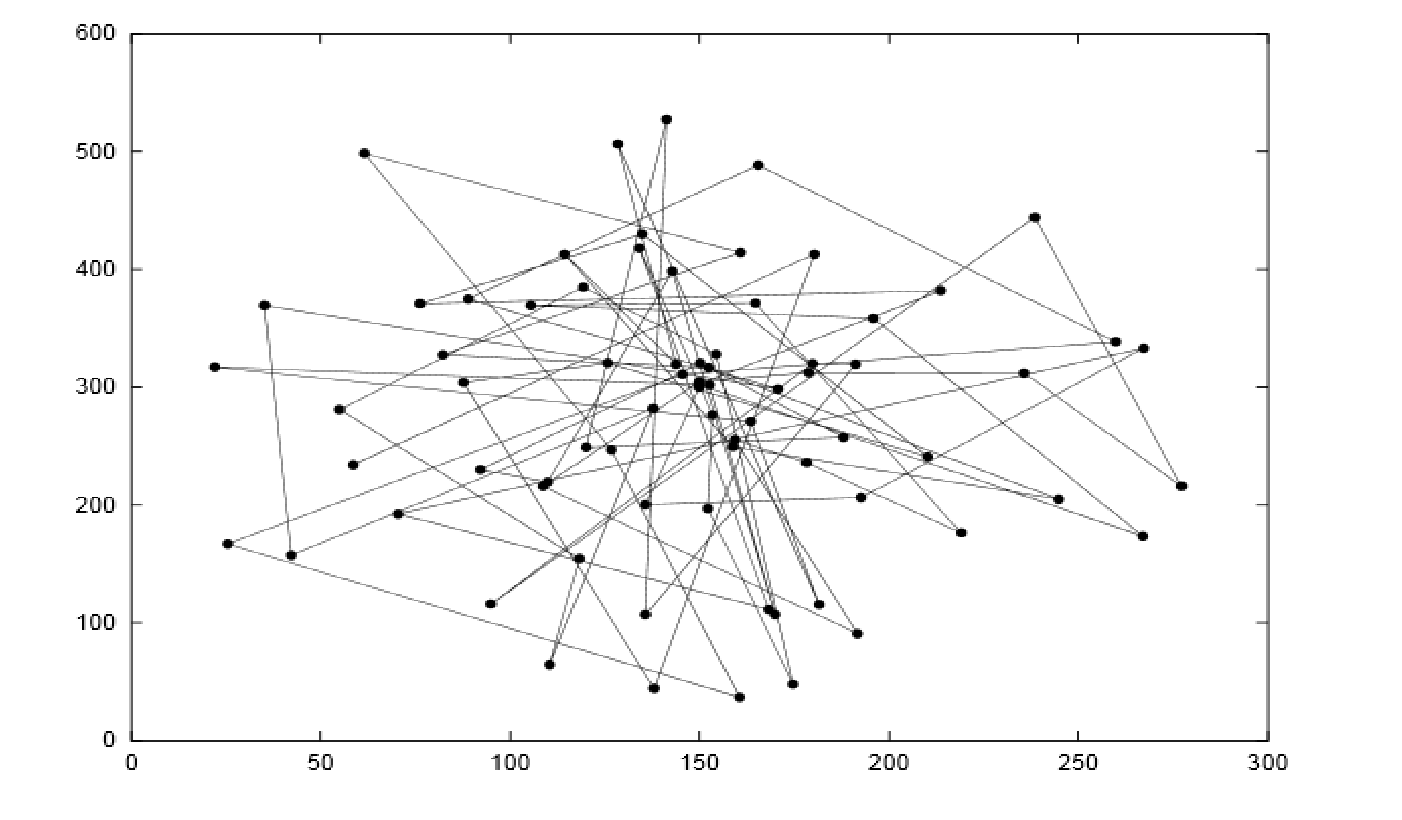
\includegraphics[width=7cm,height=50mm]{../images/randomwalk1.png}
\caption{\label{RandomWalk}Resulting pattern of a MN using the Random Walk Mobility Model}
\end{figure}


\textbf{METTRE DES SCHEMA ET DECRIRE PLUS...et maintenant?}

\subsection{Random Waypoint}

It includes pause times between changes in direction and/or speed.Once this time expires, the MN chooses a random destination and a speed, that is uniformly distributed between [minspeed, maxspeed].\\ The movement pattern of a MN who uses the RWaypointMM is similar to the RWalkMM if pause time is zero and [minspeed, maxspeed] = [speedmin, speedmax]. The Figure \ref{RandomWaypointFig} shows an example of the resulting pattern from the Random Waypoint Mobility Model.

\begin{figure}[h]
\center
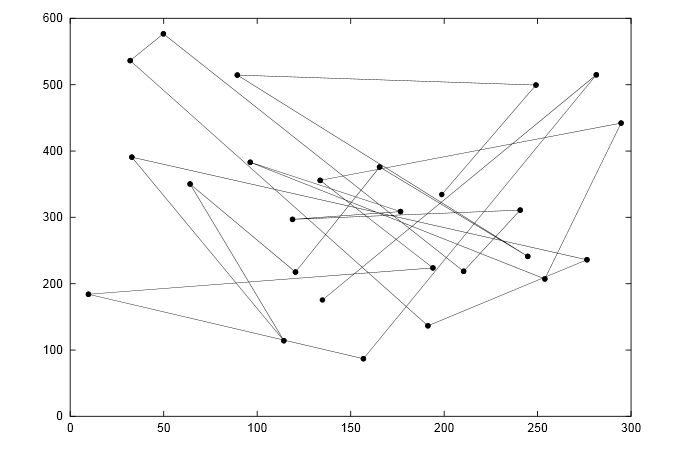
\includegraphics[width=7cm,height=50mm]{../images/randomwaypoint1.png}
\caption{\label{RandomWaypointFig}Resulting pattern of a MN using the Random Waypoint Mobility Model}
\end{figure}

During a run, MNs are initially distributed randomly around the simulation area. Figure \ref{RandomWaypointFig2} shows the average MN neighbors percentage of the MNs.\\ For example, if there are 50 MNs in the network and a node has 10 neighbors, then the node's current neighbors percentage is 20\%. Moreover, during the first 600 seconds, due to initially distributed randomly of the MNs around the simulation area, there is an high variability in the average MN neighbors percentage.\\
In the paper, there is presented three possible solutions to avoid this initialization problem.\\ 
The first is to save the location of the MNs after the initial high variability and use this position as the initial starting point of the MNs in all future simulations.\\ 
Second, initially distribute the MNs in a specific area to be a distribution more common the model, like fore example, initially placing the MNs in a triangle distribution.\\ 
Lastly, discard the initial 1000 seconds of simulation time in each simulation trials, to ensure that the initialization problem is removed even if the MNs move slowly. But if the MNs move fastly, we can discard fewer seconds of simulation time. This third solution ensures that each simulation has a random initial configuration.\\
Figure 5 : there is a complex relationship between node speed and pause time. A scenario with fast MNs and long pause times actually produces a more stable networks than a scenario with slower MNs and shorter pause times. Hence, long pause times(over 20 seconds) produce a stable network even at high speeds.

\begin{figure}[h]
\center
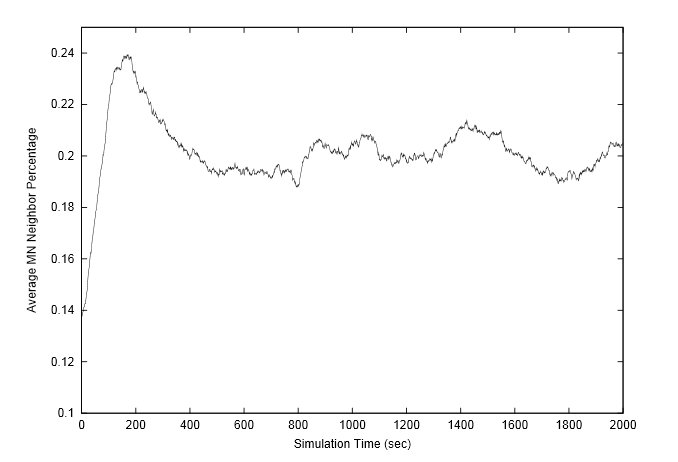
\includegraphics[width=7cm,height=50mm]{../images/randomwaypoint2.png}
\caption{\label{RandomWaypointFig2}Average neighbor percentage vs. time}
\end{figure}

\textbf{METTRE DES SCHEMA ET a revoir}

\subsection{City section}

The aim of this model is to propose a realistic model. It bases on the vehicle's movement on road maps. The specificity of this model is the map depends on each geographical zone. Here, vehicles are mobile nodes.\\\\

The mapping data blocks are available from the office Americans of the census. The map information is retrieved from text files. These files are composed of several elements:

\begin{itemize}
\item The unique identifier for a specified road.
\item The nature of the road: it can be a highway or a street.
\item The longitude of the start of position.
\item The latitude of the start of departure
\item The latitude of arrived.
\item The longitude of arrived.
\end{itemize}

All the intersections of the map are represented by nodes not mobile.
This model also considers the volume of traffic : more traffic, the more the line representing the road will be thick.
This model is also sensitive at the speed of cars (depending in particular on the hour). For example, we can consider that the speed of vehicular traffic in the morning is much smaller than at the beginning of the afternoon.\\\\

Here is the progress of this model. Every node begins in a point chosen randomly and its destination is chosen also randomly. The strategy of every node is to look for the shortest way until the destination. To achieve it, the algorithm of Dijkstra is used. Several parameters has to be considered in this algorithm as the speed or the traffic. This route can be dynamically changed. When a node reachs its destination, it begins again all the process described previously. Concerning the node's speed, it is limited to more or less 5\% of the speed registered in the file.\\
For example, here is a representation of the model. We see here that the traffic is little sparse, but with very different speeds.

\begin{figure}[h]
\center
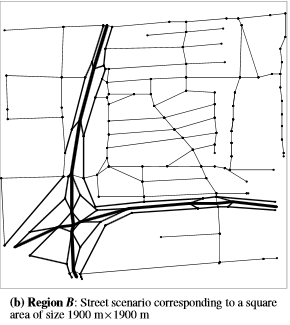
\includegraphics[width=7cm,height=50mm]{../images/city.png}
\caption{City application}
\end{figure}

\textbf{METTRE DES SCHEMA ET a compléter}

\subsection{Pheromone}

\subsubsection{Description of the model}
This model is inspired by real pheromone. A pheromone is a chemical substance, secreted externally by certain animals, such as insects, affecting the behaviour or physiology of other animals of the same species.\footnote{\url{http://dictionary.reference.com/browse/pheromone?s=t}}
\\
This model use digital Pheromone.This pheromone have 3 properties :

\begin{itemize}
\item  Deposited and withdrawn pheromone from an area. (Information fusion and aggregation).
\item  Evaporated over time. (Forget old information = Truth maintenance).
\item  Propagated from a place to its neighboring places. (Information diffusion and dissemination). 
\end{itemize}

A  digital  pheromone  represents  information  about  the  system. Different  "flavors"  of  pheromones convey different kinds of information.\\ We can have for example, attractive pheromone or repel pheromone. The attractive pheromone will attract other UAVs whereas the repel pheromone will repulse other UAVs.Digital pheromones exist within in an artificial space called a pheromone map.

\subsubsection{Scenario possible}
Pheromone logic  can  be  used  for  several  types  of  surveillance  and target  acquisition  and  tracking scenarios.\\
\begin{itemize}
\item Surveillance and Patrol
\begin{figure}[h]
\center
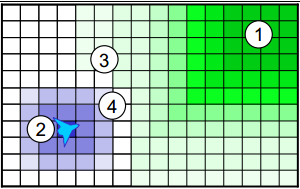
\includegraphics[scale=0.7]{../images/pheromone_surveillance.png}
\caption{\label{surveillance}Attractive and repulsive pheromones for surveillance}
\end{figure}\\\\
In Figure \ref{surveillance}, each step mean :\\
 1. Surveillance area deposits attractive pheromone,\\
 2. UAV deposits repulsive pheromone,\\ 
 3. Pheromone infrastructure propagates both attractive and repulsive pheromone to form gradient,\\
 4. UAV climbs net gradient, withdrawing attractive pheromone.
\item Target Acquisition
\begin{figure}[h]
\center
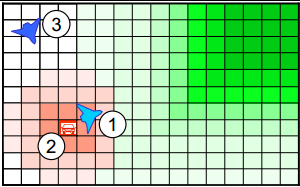
\includegraphics[scale=0.7]{../images/pheromone_target_acquisition.png}
\caption{\label{targetacquisition}Pheromones attracting confirming sensors}
\end{figure}\\\\
In Figure \ref{targetacquisition}, each step mean :\\
1. UAVdet detects target and Red target is created,\\
2. Red target deposits “NeedsID” pheromone, \\
3. UAVid is more attracted to NeedsID pheromone than lawn pheromone and 
climbs gradient to ID target. 
\item Target Tracking
\begin{figure}[h]
\center
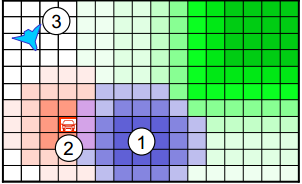
\includegraphics[scale=0.7]{../images/pheromone_tracking.png}
\caption{\label{tracking} Pheromone tracking algorithm}
\end{figure}\\\\
In Figure \ref{tracking}, each step mean :\\
1. UAV acquires target and large Visited pheromone deposit repelling 
other UAVs,\\
2. Red target estimates movement, deposits “Tracking” pheromone that eventually overcomes strength of Visited pheromone, \\
3. Nearby UAV is more attracted to Tracking pheromone than repelled by Visited pheromone and climbs gradient to reacquire the target. 
\end{itemize}
\subsubsection{Real scenario}

We are going to see a real scenario wich demonstrate the use of pheromone model.\\
The demonstration used: 
\begin{itemize}
\item Four robots 
\item A mock urban area  
\item Two UAVs controlled by pheromone technology 
\end{itemize}

\textbf{A CHANGER LE TEXTE CI DESSOU}
The demonstration focused on the swarming algorithms that control and coordinate the behaviors of the heterogeneous mix of vehicles.  
Pheromone  algorithms  controlled  and  coordinated  the  flight  of  the  two  UAVs  as  they  performed 
continuous  surveillance  over  an  urban  area  looking  for  potential  adversaries.  The  two  air  units 
worked together to ensure even, thorough, and continuous coverage of all areas in the surveillance 
region  while  avoiding  any  collisions.  They  also  provided  patrol  coverage  of  a  mock  convoy  as  it 
moved through the area. 
While the UAVs surveyed a broad area over the airfield, the ground robots surveyed and patrolled 
around  some  mock  buildings  set  up  for  the  demo.  During  the  demonstration,  one  of  the  ground 
robots  failed.  The  other  ground  robots  were  able  to  dynamically  readjust  their  patrol  patterns to 
accommodate  the  missing  unit  without  any  intervention  by  the  operator.  This  unplanned  event 
helped to demonstrate the robustness of these algorithms to unexpected events. 
The  demonstration  showed  cooperative  behavior  between  the  air  and  ground  units  when  the 
identity of a potential adversary detected by one of the UAV’s was automatically confirmed by one of 
the ground robots with a special sensor capable of target identification. 
The operator simply gives a high level command to the whole swarm, such as “survey this area and 
track  any  identified  targets”  or  “patrol  around  this  convoy”.  The  robots  autonomously  configured 
themselves to determine which robot would perform what task in order to accomplish the overall 
objective.  


\subsection{Natural Agent}

\subsubsection{Ants}

Le modèle de mobilité des fourmis se base sur le fait que les fourmis construisent des réseaux de sentiers qui relient leurs   nids avec des sources de nourritures disponible.
Chaque fourmi qui se nourrit à le même programme :

\begin{itemize}
\item Elle doit éviter les obstacles.
\item Aller ou elle veut (déplacement aléatoire) tant qu'il n'y a pas de phéromones.
\item Si elle arrive à trouver de la nourriture, elle laisse des phéromones pendant un temps t pour pouvoir indiquer aux autres fourmis l'emplacement de la nourriture.
\item Si la fourmi trouve de la nourriture, elle l'a ramène à son nid.
\end{itemize}

Les fourmis peuvent mourir. Soit elles ne trouvent pas de la nourriture assez rapidement et meurt de faim, soit elles se font tuer par d'autres prédateurs.
Tous les chemins de phéromones conduisent à de la nourriture. Mais les phéromones s'évaporent dans le temps. Le taux de phéromone peut être renforcé si plusieurs fourmis passent par le même chemin.

\textbf{METTRE DES SCHEMA ET a compléter}

\subsubsection{Termites}

\subsubsection{Wasps}

le modèle basé sur les guêpes est composé de plusieurs caractéristiques :
\begin{itemize}
\item un chef qui répartit les différentes guêpes dans différents groupes
\item 
\end{itemize}

\subsection{Birds and Fish}

\subsection{Wolves}

\newpage
\section{Scenarios}

\newpage
\section{Needs Analysis}
\subsection{Functional Requirements}


\subsection{Non-Functional Requirements}
\newpage
\chapter{Architecture}


\newpage
\chapter{Schedule}
\section{Tasks List}

\section{PERT}

\section{GANTT}
\newpage
\chapter{Works Done}
\section{What we did}
Durant les deux mois et demi de ce projet, nous avons implémenté les deux modèles qui étaient décrit dans l'article. Pour rappel, ces deux modèles sont un random simple et un modèle concernant des phéromones. Dans cette rubrique, nous allons vous expliquer le travail de développement que nous avons fourni et les différents choix effectués. Nous n'avons pas trouvé d'utilité à faire un diagramme UML vu la simplicité de l'architecture.\\\\

During two and a half months of this project, we implemented both models which were described in the article. As a reminder, these two models are a simple random and a model concerning pheromones.We also implemented the Random Waypoint model on the demand of our customers. In this section, we are going to explain you the work of development which we supplied and the various made choices. We did not find utility to make a UML diagram seen the simplicity of the architecture.\\\\

\subsection{random model} 

Pour implémenter ce modèle, nous avons eu besoin de trois classes.\\
La première classe, qui se nomme Main.java, permet comme son nom l'indique de lancer le programme. C'est dans cette classe que nous définissons la taille de la fenêtre, la matrice qui servira à simuler le scan d'une zone (tous les noeuds auront la même matrice), et l'instanciation des différents objets provenant de la librairies JBotSim. Nous avons par exemple, un objet s'intitulant \textit{topo} qui est une topology. Cet objet est la base pour notre simulateur. C'est à cette topology que l'on va pouvoir ajouter des nœuds mobiles (ici des avions).\\

To implement this model, we needed three classes. \\
The first class, which is called \textit{Main.java}, allows as its name indicates it launching the program. It is in this class that we define the size of the window, the matrix which will serve to feign the scan of a zone (all the nodes will have the same matrix), and the instanciation of the various objects coming of JBotSim library. We have for example, an object being entitled \textit{topo} which is a topology. This object is the base(basis) for our simulator. It is to this topology that we are going to be able to add mobile nodes (here planes). \\

Nous avons aussi instancié un objet de type Jtopology. Nous expliquerons ce choix dans la suite de la présentation des classes.\\\\
La deuxième classe de notre architecture se nomme \textit{MovingNode}. C'est dans cette classe que sera traité le mouvement des différents nœuds. Cette classe hérite donc de la classe \textit{Node} et implémente l'interface \textit{ClockListesner}, toutes les deux provenant de la librairie JBotSim. Elle hérite de la classe \textit{Node} car les avions seront représentés par des nœuds mobiles, il nous faut donc les caractéristiques de ceux-ci. De plus, elle implémente l'interface \textit{ClockListener} car nous avons besoin que nos nœuds bougent tout les certains temps, on a donc besoin d'un clock d'horloge pour réaliser cela. Nous aurons donc un listener pour le temps, ainsi qu'une méthode \textit{onClock} qui sera appelée à chaque top d'horloge.\\\\

We also instantiated an object Jtopology's object type. We shall explain this choice during the presentation of classes. \\\\
The second class of our architecture is called \textit{MovingNode}. It is in this class that will be handled the movement of the various nodes. This class thus inherits from the class \textit{Node} and implement the interface \textit{ClockListesner}, both resulting(coming) from the JBotSim. It inherits from the class \textit{Node} because planes will be represented by mobile node, we thus need the characteristics of these. Furthermore, It implements the interface \textit{ClockListener} because we need that our nodes move all the seconds, we thus need a top of clock to realize it. We shall thus have a listener for time , as well as a method \textit{onClock} which will be called to every top of horloge. \\\\


Cette classe contient un constructeur par défaut, permettant d'instancier et d'initialiser les différents variables, et d'associer des images aux noeuds mobiles (appel de la méthode \textit{setProperty}. Le modèle random a pour caractéristique de n'avoir aucune communication entre les différents noeuds. Pour réaliser cela, nous passons un argument valant \-1 à la méthode \textit{setCommunicationRange}.\\\\
Comme indiqué dans l'article, les noeuds du modèle random changent d'actions toute les secondes en fonctions de la dernière action entreprise. Pour rappel, voici la table d'action pour le modèle random : \\\\

This class contains a constructor by default, allowing to instantiate and to initialize the various variable, and to associate images with the mobile nodes (call of the method \textit{setProperty}. The random model has for characteristic to have no communication between the various nodes. To realize it, we cross a being worth argument \-1 in the method \textit{setCommunicationRange}. \\\\
As indicated in the article, the nodes of the random model change actions quite the seconds in functions of the last undertaken action. As a reminder, here is the table of action for the random model: \\\\
\begin{center}
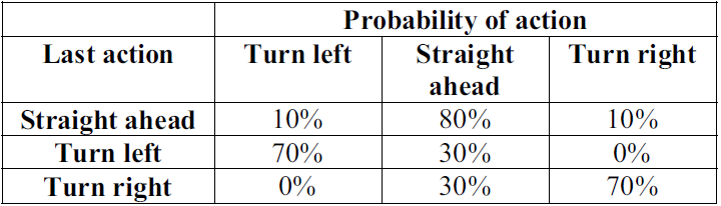
\includegraphics{../images/table_random.png}
\end{center}

Dans notre implémentation, nous avons donc une variable \textit{lastdirection} permettant de savoir la dernière action qui a été faite. Nous avons associé des chiffres aux dernières actions de faite. Si la dernière direction était la gauche, alors la variable \textit{lastdirection} prend la valeur 1, si elle était tout droit, alors on lui associe la valeur 2, et si c'était à droite, on lui associe la valeur 3.\\\\

In our implementation, we have a variable \textit{lastdirection} allowing to know the last action which was made. We associated figures with the last actions of made. If the last direction was the left, then the variable \textit {lastdirection} takes the value 1, if it was quite right, then we associate the value 2, and if it was to the right, we associate the value 3. \\\\

Pour respecter le plus possible la réalité, nous avons dû modifier la gestion des bords de la fenêtre. En effet, à l'origine dans JBotSim, les noeuds peuvent passer d'un bord à l'autre. Par exemple, s'ils atteignaient le bord gauche, ils se retrouvaient par la suite à droite de la fenêtre, ce qui n'est pas possible dans la vie réelle. Nous avons donc bloqué ce problème en rectifiant les coordonnées du noeud, et en changeant son angle de direction. \\\\

To respect as much as possible the reality, we had to modify the management of the edges of the window. Indeed, originally in JBotSim, nodes can pass from an edge to the other one. For example, if they reached the left edge, they found themselves afterward to the right of the window, what is not possible in the real life. We blocked this problem by rectifying the position of the node, and by changing its angle of direction. \\\\

A chaque fois qu'un noeud scanne une zone, il regarde dans la matrice si cette position a déjà été scanné (0 si la zone n'a jamais été scanné, 1 sinon). Si c'est le cas, alors il ne fait rien, sinon il met la valeur à 1.\\\\

La troisième classe de notre architecture se nomme \textit{Jtopology\_Random}. Elle hérite de JTopology et va permettre de dessiner les traces des scans sur la map. Cette classe JTopology hérite de JPanel, et se situe en fait entre une JViewer et une Topology.\\\\

Every time a node scans a zone, it looks in the matrix if this position was already scanned (0 if the zone was never scanned, 1 otherwise). If it is the case, then it makes nothing, otherwise it puts the value to 1. \\\\

The third class of our architecture is called \textit{Jtopology\_Random}. It inherits from JTopology and is going to allow to draw the tracks of scans on the map. This class JTopology inherits from JPanel, and is situated in fact between a JViewer and a Topology.

\subsection{Random Waypoint Model}

This model is very similar to the previous. The only difference is their way to move. \\In this model, the node choose one point randomly and move to it. \\So the only modification compared to the previous model is the class \textit{MovingNode} and more precisely the method \textit{on clock}.


\subsection{Pheromone model}
Au niveau architecture, l'implémentation du modèle des phéromones est très similaire. On retrouve pratiquement les 3 même classe. Seulement la classe \textit{MovingNode} va réellement être différente car les mouvements des noeuds vont dépendre de beaucoup de paramètre. Tout d'abord, cette classe implémente une interface de plus qui est \textit{MessageListener}. En effet, dans ce modèle, les noeuds vont devoir se transmettre des données (en l'occurrence leur map respective).\\\\

La méthode qui va changer le plus par rapport au modèle aléatoire est la méthode \textit{onClock}. En effet, c'est ici que l'on va appliquer les règles comme décrites sur l'image suivante : \\\\

Concerning the architecture, the implementation of the model of pheromones is very similar. We find practically 3 even classy. Only the class \textit{MovingNode} is really going to be different because the movements of nodes are going to depend on a lot of parameter. First of all, this class implements an interface furthermore which is \textit{MessageListener}. Indeed, in this model, nodes are going to have to be passed on data (in this particular case their respective map). \\\\

The method which is going to change most with compared with the random model is the method \textit{onClock}. Indeed, it is here that we are going to apply rules as described on the following image:

\begin{center}
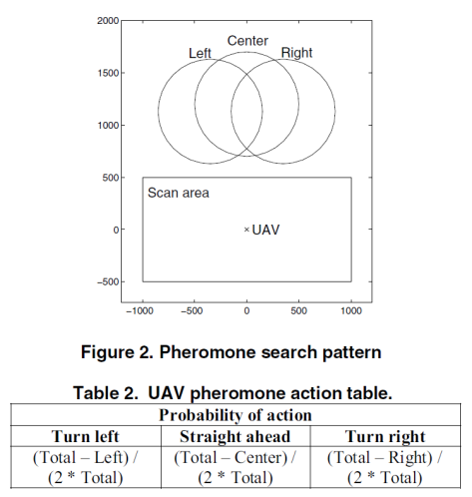
\includegraphics{../images/pheromon_model.png}
\end{center}

Nous avons traité tous les cas décrits dans l'article, c'est à dire que le noeud regarde les valeurs des phéromones en diagonale gauche, devant lui, en diagonale droite.\\\\

Une autre caractéristique de notre implémentation est que cette fois-ci, nous ne scannons plus un point de la carte mais les 5 décrits précédemment.\\\\

We handled all the cases described in the article, that is the node looks at the values of pheromones in its left diagonal, in front of him and in its right diagonal.

\begin{figure}[h]
\center
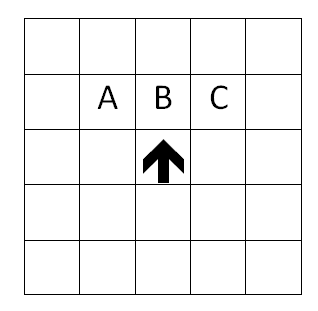
\includegraphics[width=5cm]{../images/grille_case_1.png}
\caption{case 1}
\end{figure}

\begin{figure}[h]
\center
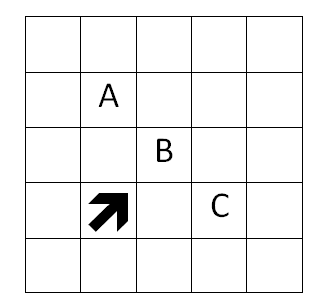
\includegraphics[width=5cm]{../images/grille_case_2.png}
\caption{case 2}
\end{figure}

These both case show how a node scan the map.
\begin{itemize}
\item the area A represents the left diagonal of the node.
\item the area B represents the front of the node.
\item the area C represents the right diagonal of the node.
\end{itemize}

Another characteristic of our implementation is that this time, we do not scan any more a point of the map but 5 described previously  like the picture below.

\begin{figure}[h]
\center
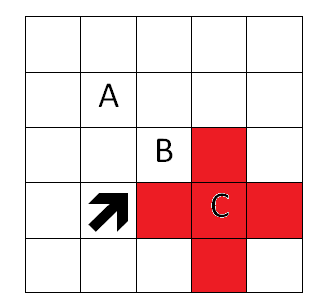
\includegraphics[width=5cm]{../images/grille_case_2_scan.png}
\caption{scan of area C}
\end{figure}

\textbf{A COMPLETER}



\section{Difficulties Encountered \& Solutions}

Au niveau de l'implémentation, nous n'avons pas rencontré beaucoup de difficultés. Le seul gros problème est l'affichage des zones scannées. Sur les conseils de Monsieur Casteigts, nous avons dû créer une classe héritant de JTopology et redéfinir la méthode \textit{paint}. En effet, le rafraichissement de l'affichage des zones scannées est un problème car nous perdions les zones scannées précédemment. Nous avons donc créé une ArrayList pour sauvegarder les zones scannées pour les redessiner à chaque fois.\\\\

La plus grosse difficultés rencontrées a été la lecture des nombreux articles en correspondance avec notre article d'étude. Ils comportaient de nombreuses pages et la lecture de ceux-ci en Anglais nous a prit énormément de temps. Nous avons dû par la suite mettre à jour les articles lus en recherchant sur internet les mises à jour.

Concerning the implementation, we did not meet many difficulties. The only big problem is the display of the scanned zones. On the advice of Mister Casteigts, we had to create a class inheriting from JTopology and redefine the method \textit{paint}. Indeed, the refreshment of the display of the scanned zones is a problem because we lost zones scanned previously. We created a ArrayList to save area scanned to redraw them in every times. \\\\

\newpage
\part{Observations}
\setcounter{chapter}{0}
\chapter{Results}

\section{The article}

\subsection{Scan Coverage}

The goal of the UAVs is to scan the full map once per hour. In theory, with a speed of 150 km/h, the maximum scan speed is 0.083 km\textsuperscript{2}/second/UAV. So with an area of 900 km\textsuperscript{2}, the fastest time to cover the full area is 18 minutes. The figure \ref{randomcoverage} and the figure \ref{pheromonecoverage} represent the coverage data from the mobility models.

\begin{figure}[h]
\centering
   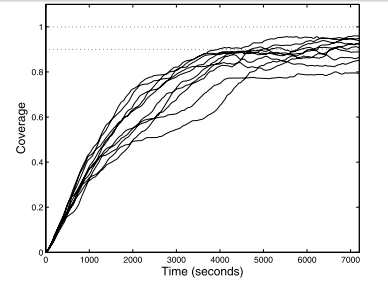
\includegraphics{../images/random_coverage.png}
   \caption{\label{randomcoverage} Random mobility coverage\cite{UAV}}
\end{figure}

\newpage

\begin{figure}[!h]
   \centering
   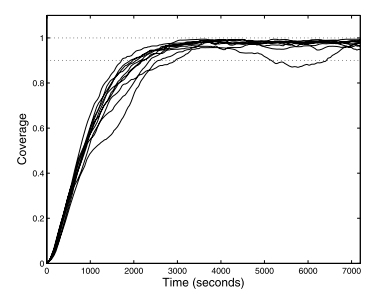
\includegraphics{../images/pheromone_coverage.png}
   \caption{\label{pheromonecoverage} Pheromone mobility coverag\cite{UAV}}
\end{figure}

For the random model, we see that it need more than 83 minutes to reach 80 percents of coverage. Whereas the pheromone model reach the 90 percents in 60 minutes. Comparing the two models, the pheromone model has a much higher coverage rate.

\subsection{Scan Characteristic}

In Figure \ref{randomchar} and Figure \ref{pheromonechar}, the solid lines represent the probability distribution of each models. This curve permits to calculate the probability of the next scan.\\
To know the probability of the next scan between the time t1 and t2, we have to calculate the area under the curve between t1 and t2.\\
So to meet with the requirement of one scan of the map per hour, the curve must be 0 at 1 hour. However none models reach 0 before one hour, because no model manages to achieve full coverage, the pheromone model manages well to avoid rescanning a recently scanned area. We can see that on the graphic : the median curve follows the dashed line at time between 0 seconds and 1000 seconds.

\newpage

\begin{figure}[!h]
\centering
   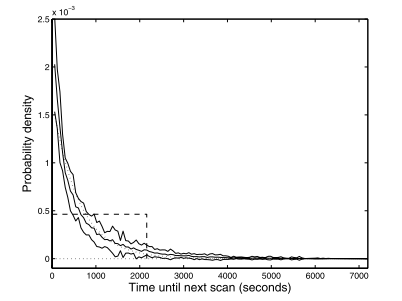
\includegraphics{../images/random_scan_characteristic.png}
\caption{\label{randomchar} Random mobility\cite{UAV}}
\end{figure}

\begin{figure}[!h]
   \centering
   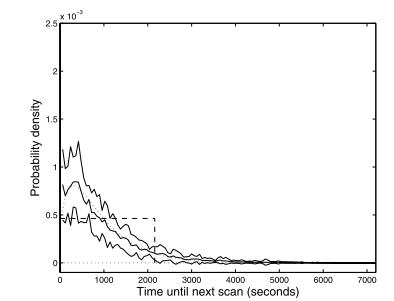
\includegraphics{../images/pheromone_scan_characteristic.png}
\caption{\label{pheromonechar} Pheromone mobility\cite{UAV}}
\end{figure}

\subsection{Never scanned area}

In this table below, we can see the results about the percentage of the map never scanned.\\

\begin{center}
\begin{tabular}{|c|c|c|c|}
\hline
	      & Max & Median & Min \\
	      \hline
	Random & 16.2\% & 3.2\% & 0.5\% \\
	\hline
	Pheromone & 0.21\% & 0.03\% & 0.01\% \\
	\hline
\end{tabular}
\end{center}

It represents the maximum, median and minimum uncovered area for the ten runs. These numbers clearly show the ability of the pheromone model to cover the complete area. 

\newpage

\subsection{Connectivity}

\begin{figure}[!h]
   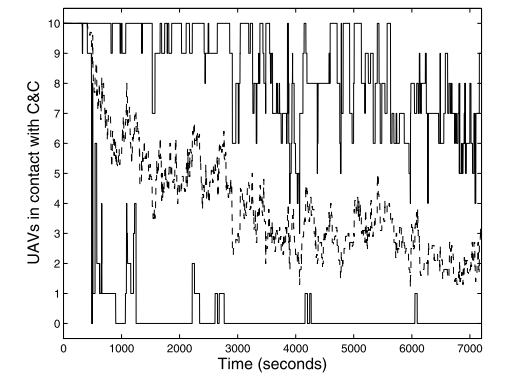
\includegraphics{../images/random_resultat_connectivite.png}
\caption{\label{randomconnect} Random. Number of UAVs in contact with C\&C (max, average, min)\cite{UAV}}
\end{figure}

\newpage

\begin{figure}[!h]
   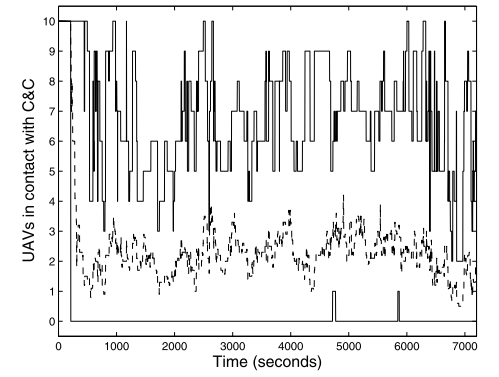
\includegraphics{../images/pheromone_resultat_connectivite.png}
\caption{\label{pheromoneconnect}Pheromone. Number of UAVs in contact with C\&C (max, average, min)\cite{UAV}}
\end{figure}

In Figure \ref{randomconnect} and Figure \ref{pheromoneconnect},we can see the number of UAV wich can communicate with the C\&C.  The  graphs  show the maximum, average, and minimum of this number for the ten runs. We saw that both models don't provide good connectivity. There are not enough UAV to have a fully connected communication graph. Because of the pheromone logic that pushes the UAVs away from each other, this model have low connectivity. Whereas the random model have a high connectivity at the beginning of the run. Then with the random trajectory of each UAV, they move away from each others and finally this model finishes to have the same poor connectivity as the pheromone model.

\section{Our Implementation}

\subsection{Scan coverage}

The graphic \ref{scancoverage} is the result of our experiments using our implementation of the random walk and waypoint mobility model and the pheromone mobility model. Each run lasts 20 minutes and uses 10 UAVs per model.

\begin{figure}[!hbtf]
\centering
   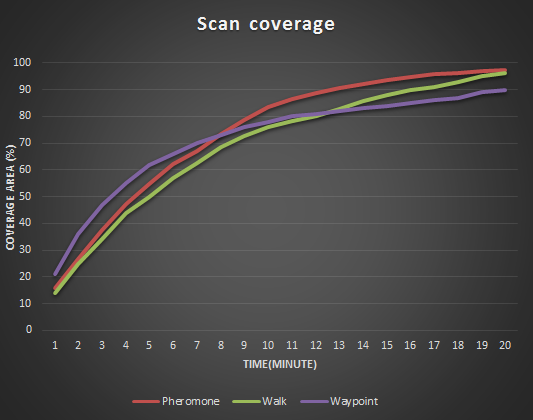
\includegraphics{../images/ScanCoverageResult.png}
\caption{\label{scancoverage} Scan coverage resulting of our implementation}
\end{figure}

\begin{itemize}

\item Observation

We can see that the random waypoint mobility model covers a higher scan area until 7 minutes than the others mobility models. From 7 minutes to the end, the better mobility model is the pheromone one. The random walk is in third position until 13 minutes, at this time, this is the random waypoint becomes the third. At the end of the run, the random waypoint doesn't exceed 90\%, the random walk rises approximatly to 95 \% and the pheronome model a little bit.

\item Interpretation

The random waypoint is better to reach a higher percent of scanned area because each UAV chooses a destination and travels to. But at a moment, the most part of the time, the UAVs pass again on an area already scanned. Hence the random waypoint can't target 100\% in a reasonable time.

The random walk is slower than the others models because each UAV changes its destination each second. But at the end of the simulation, this model reaches over 90\% like the pheromone model. Indeed, this model takes a long time to disperse each UAV all over the map.

The pheromone model quickly distributes all the UAVs over the map because the UAVs repel others. So this model is more efficient than the random walk. But, at the beginning of the run, the random waypoint is more efficient than pheromone model because this one include a part of random mobility model in the moving of each UAV. Each of them change its direction every second. Finally, the percent of scanned area increases progressively.

\item Conclusion

The pheromone mobility model is the better model to reach quickly the most percentage of scanned area. Indeed, the random mobility models aren't appropriate to scan the entire area.

\end{itemize}


\newpage
\section{Tests}


\newpage
\chapter{Improvements}

\section{Mobility models}

\begin{itemize}

\item In this article, they use The pheromone repel model wich had a bad connectivity. To improve the connectivity, we can add attractive pheromone. At regulary time, the C\&C can add attractive pheromone in its place to force the UAVs to move to it. So we have a regulary update of the full map.

\item An other way to improve this model is to add more C\&C on the area. Therefore each UAV has a map more often update.

\item We can also give a area to each UAV. To do that we can add attractive pheromone in different area for each UAV. So each UAV scan their area and move to the C\&C.

\item We can increase highly the connectivity adding others small UAV wich could maintain the communication with the C\&C. These small UAV can make the communication path between an UAV and the C\&C. 

\end{itemize}



\newpage
\chapter{Development Environment and Conventions}

In this part, we will see the development environment we used, and the programming conventions we've applied.

\section{Development Environment}

\subsection{github}

To write this report and to be able to implement both models most effectively possible, we used a tool of hosting and management of program which is called Github. It is a tools of versionning which allows the collaborative work and allows a simplification of the methods of work.\\
We used it throughout the project to put the summaries of articles that we read, the tasks which we had to make, this report or still the implementation.\\
Our Git repository is located at the following address : \\
\url{https://github.com/jetcheve/M2\_PER\_MMUAVGRA}.\\

Our deposit decomposes into three branches :

\begin{itemize}
\item A master branch which is general to the whole deposit.
\item A branch called Develop. It is in this branch that there will be all the code for implementing different models. It also contains a test folder. 
\item An branch report, which as its name suggests, contain all the parts of our report and the pictures have inside it.
\end{itemize}

\subsection{Eclipse}

Eclipse is an integrated development environment for creating projects in any programming language. It is used to develop programs in JAVA, Android, C, etc.\\

We used Eclipse throughout the project implementation.\\

As a supplement to Eclipse, we used a library that is called JBotsim \cite{JBotSim} proposed by Mr. Casteigts. This allows to simulate a dynamic network. This network is simulated with mobile nodes that interact. These nodes can send messages (in our case, maps of each UAVs).\\

We used this library because it is very easy to use, and it adapt well to the needs which we had.

\section{Programming Conventions}

First, we've choosed to used the Java Coding Conventions, which we can see in the following link \url{http://www.oracle.com/technetwork/java/codeconventions-150003.pdf}\\

Then, in order to create our documentation, we've used the Doxygen Convention, viewable here \url{http://www.stack.nl/~dimitri/doxygen/manual/docblocks.html}\\
We've relied heavily on this documentation and have mostly employed these protocoles below.\\

\lstset{language=Java,basicstyle=\footnotesize,commentstyle=\color{blue}}
\begin{lstlisting}[frame=trBL, title=Doxygen Convention for classes]
/**
* @class name of the class
* @brief Description of herself
*/
\end{lstlisting}

\lstset{language=Java,basicstyle=\footnotesize,commentstyle=\color{blue}}
\begin{lstlisting}[frame=trBL, title=Doxygen Convention for methods]
/**
* @brief Description of the method
* @param the parameters and their descriptions
* @return the description of what return the method (optional)
*/
\end{lstlisting}

\lstset{language=Java,basicstyle=\footnotesize,keywordstyle=\color{red},commentstyle=\color{blue}}
\begin{lstlisting}[frame=trBL, title=Doxygen Convention for members]
int var; /**< Detailed description after the member */
\end{lstlisting}
~\\

We've also resorted to programming conventions that we defined between us.\\
For example, when a part of a code, was not finished yet, we put the following lines above the concerning part.\\\\\\\\

\lstset{language=Java,basicstyle=\footnotesize,commentstyle=\color{blue}}
\begin{lstlisting}[frame=trBL, title=Programming convention for unfinished code]
/**
* @TO_DO
* Description
*/
\end{lstlisting}
~\\

We've also used a convention for the bugs found and wrote these protocoles, depending on whether the bug was resolved or not.\\
We used it, in line with the Bug Tracking of GitHub.\\

\lstset{language=Java,basicstyle=\footnotesize,commentstyle=\color{blue}}
\begin{lstlisting}[frame=trBL, title=Programming convention for bugs]
/**
* @BUG
* @Unfinished/finished
* Description
*/
\end{lstlisting}
~\\

To finish, we've created the five essential files for a project :\\

\begin{itemize}
\item INSTALL.txt  : Installation instructions for the project,
\item LICENCE.txt  : Licence and copyright \copyright{} of the project,
\item README.txt   : General description of the project,
\item AUTHORS.txt  : Authors of the project,
\item MANIFEST.txt : Tree structure and files list of the project.
\end{itemize}

\newpage
\chapter{Conclusion}
\newpage
\addcontentsline{toc}{section}{Bibliography}
\nocite{*}
\bibliographystyle{unsrt}
\bibliography{bibliography}

\end{document}

